\documentclass[a4paper,12pt]{report}
\usepackage{graphicx}
\title{Tugas Besar Database}
\author{Nuha Hanifatul Khonsa' 1184085}
\date{18 Desember 2019}
\begin{document}


\maketitle


\section{Langkah Dalam Membuat Aplikasi Stok Barang Pada Toko Aksesoris Menggunakan Orecle APEX}
\par Oracle Application Express (Orecle APEX) adalah pengembangan perangkat lunak berbasis web yang berjalan pada database Oracle. Edisi Oracle Database dimulai dengan Oracle 11g, Dengan menggunakan orecle APEX kita dapat membuat aplikasi secara express atau cepat, hal ini dikarenakan pada Orecle APEX telah tersedia tool dalam membuat aplikasi. Pada 'Tugas Besar Database' ini saya akan menjabarkan mengenai 'Langkah dalam Membuat Aplikasi Stok Barang pada Toko Aksesoris menggunakan Orecle APEX tentunya.
\begin{enumerate}
    \item Sebagai langkah awal ialah memiliki aplikasi Orecle APEX, Orecle APEX dapan diakses secara online maupun offline, jika offline berarti kita harus memiliki aplikasi Orecle APEX dengan mendownload pada website orecle.com. Lalu kita dapat menginstal Orecle APEX saat proses menginstal kita akan diminta untuk mengisikan username yaitu system dan password sesuai dengan keinginan kita. Kemudian kita dapan membuat Workspace dengan skema HR dan tak lupa untuk mensetting username dan password. Pada Aplikasi Offline kita dapat membuat aplikasi dengan syarat login memasukkan workspace, username dan password seperti halnya saat kita login pada Orece APEX Online. Sedikit ada perbedaan jika kita menggunakan Orecle APEX Online kita hanya perlu melakukan registrasi pada website Orecle APEX https://apex.oracle.com/ jika kita telah memiliki akun kita dapat melakukan login langsung dengan memasukkan workspace, username, dan password. Ini adalah Halaman login Aplication Express Offline
    \begin{center}
    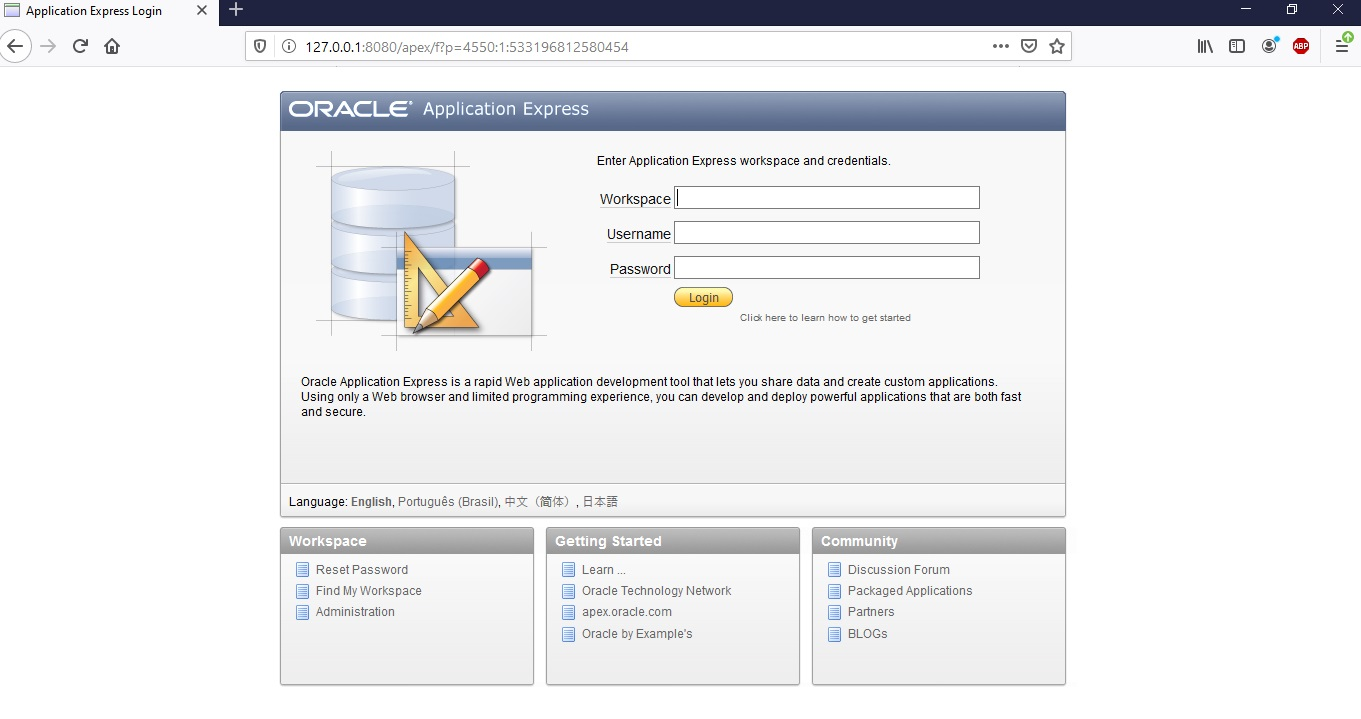
\includegraphics[width=11cm\textwidth]{figure/loginoff.jpg}
    \end{center}
    \item Pada pengerjaan Tugas Besar kali ini saya menggunakan Orecle APEX Online, Jadi Hal yang pertama saya lakukan ialah Login pada Orecle APEX online dan kebetulan saya telah memiliki akun orecle APEX jadi saya tinggal Login dengan memasukkan Workspase, Username, dan Password. Seperti Pada gambar berikut:
    \begin{center}
    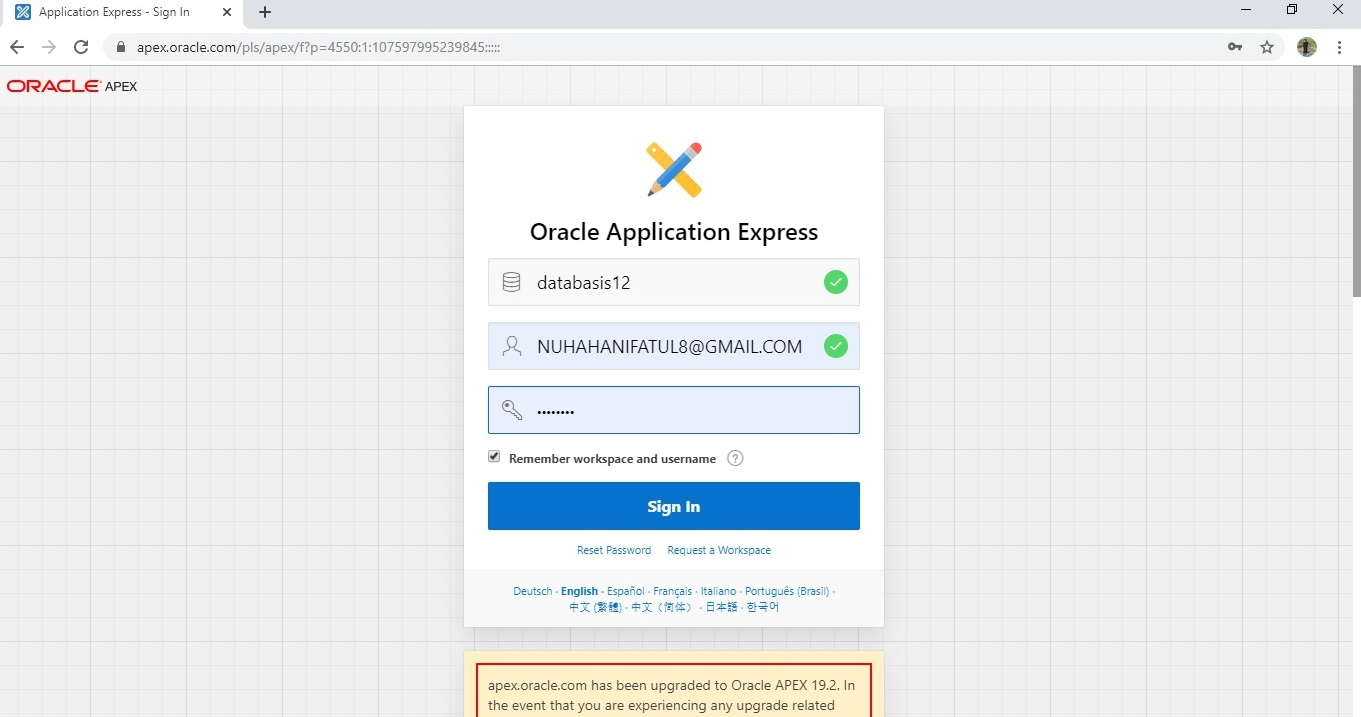
\includegraphics[width=11cm\textwidth]{figure/login.jpg}
    \end{center}
    \item Setelah kita berhasil Login lalu kita dapat memulai membuat table dengan memilih Menu SQL Workshop lalu pilih SQL Command yang berfungsi sebagai laman menuliskan query.
    \item Pada SQL Command kita dapat memulai membuat table disini saya membuat table stok. Dalam membuat table kita dapat menggunakan perintah 'create table' karena saya akan membuat table sto jadi kita dapat menuliskan 'create table stok' dan dikuti dengan isi dari table stok yaitu id produk, nama produk, dan jumlah stok, untuk primary key terletak pada id produk. Hal terpenting jangan lupa untuk run agar table terbuat dan kita tau adakah eror dari query yang telah kita ketikkan. Hal ini seperti pada gambar berikut:
    \begin{center}
    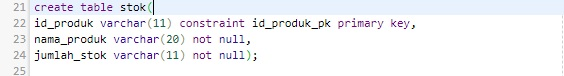
\includegraphics[width=11cm\textwidth]{figure/stok.jpg}
    \end{center}
    Setelah berhasil membuat table stok dan berhasil run kita dapat memulai membuat table selanjutnya yaitu table 'tambah produk', yang diikuti 2 kolom yaitu kode suplier, tanggal masuk, id produk, dan jumlah masuk dari barang tersebut, sedangkan untuk primary key terletak pada kode suplier. Query dapat dituliskan seperti pada gambar berikut:
    \begin{center}
    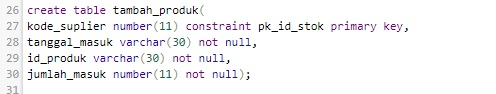
\includegraphics[width=11cm\textwidth]{figure/tambah_produk.jpg}
    \end{center}
    \item kita telah berhasil membuat table yaitu table stok dan tambah produk Nah, sekarang kita dapat mengisikan data pada tiap table menggunakan perintah insert. pertama kita akan mengisikan table stok kita dapat menuliskan Query seperti berikut ini:
    \begin{center}
    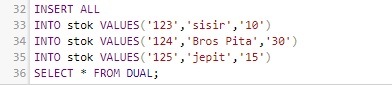
\includegraphics[width=11cm\textwidth]{figure/insertstok.jpg}
    \end{center}
    pada query diatas kita memasukkan nilai dari tiap coloum yang harus sesuai. sesuai dengan hal yang ada pada perintah kolom tersebut seperti tipe data dan length tentunya. Lalu kita dapat menginsert / mengisikan values untuk table selanjutnya yaitu table tambah produk dengan query sebagai berikut:
    \begin{center}
    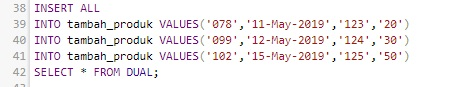
\includegraphics[width=11cm\textwidth]{figure/inserttambah.jpg}
    \end{center}
    Ketelitian menjadi hal terpenting dalam menuliskan query agar tidak terjadi eror. 
    \item Setelah kita berhasil melalukan perintah insert untuk mengisi values pada tiap table sekarang kita mempersiapkan untuk dapat melakukan perintah trigger dimana perintah trigger ialah perintah yang berfungsi sebagai perintah otomatis perubahan spesifik dimana dalam kondisi sebelum maupun sesudah eksekusi DML (Data Manipulation Language) seperti insert, update, delete. disini saya membuat table 'history tanbah produk' table ini akan dipanggil saat nanti eksekusi perintah trigger. Table 'history tanbah produk' ini berisikan kode suplier, tanggal masuk, id produk, dan jumlah masuk serta ada tambahan yaitu changed at timestamp dan changed type varchar(255). Query dapat dituliskan seperti ini:
    \begin{center}
    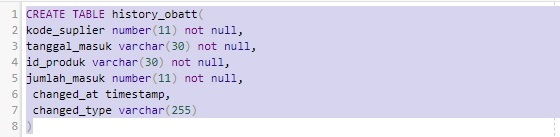
\includegraphics[width=11cm\textwidth]{figure/history.jpg}
    \end{center}
    \item Kita telah membuat table yang akan kita panggil dalam fungsi trigger. Nah, sekarang kita dapat menuliskan fungsi trigger yaitu insert, update, dan delete. pertama kita buat trigger delete dengan Query seperti ini:
    \begin{center}
    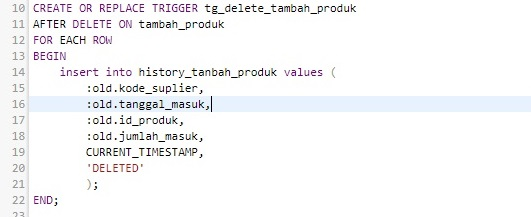
\includegraphics[width=11cm\textwidth]{figure/trigger_delete.jpg}
    \end{center}
     hal ini dapat dijabarkan bahwa kita membuat fungsi trigger dengan nama 'tg delete tambah produk' yang aka berjalan otomatis setelah di hapus atau delete pada table 'tambah produk' untuk tiap baris dimulai dengan menambahkan pada table 'history tanbah produk' dengan nilai coloum lama seperti kode suplier, tanggal masuk, id produk dan jumlah masuk yang lama dihapus. 
    kita akan membuat trigger fungsi update dengan query sebagai berikut:
    \begin{center}
    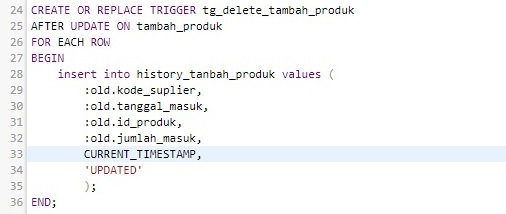
\includegraphics[width=11cm\textwidth]{figure/trigger_update.jpg}
    \end{center}
    tidak banyak yang kita ubah saat menuliskan query trigger update ini dari trigger delete tadi yaitu bergantinya perintah delete menjadi update. Hal ini dimana data yang terupdate otomatis. Sedangkan untuk fungsi trigger insert dengan sebagai sebagai berikut:
    \begin{center}
    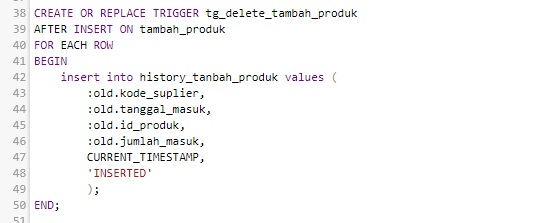
\includegraphics[width=11cm\textwidth]{figure/trigger_insert.jpg}
    \end{center}
    \item Fungsi View pada aplikasi ialah menyederhanakan table view sendiri table virtual dengan kata lain table yang sebenernya tidak ada. View berisikan kumpulan query perintah dari beberapa table. sehingga jika suatu fungsi view dipanggil tidak harus menuliskan query yang panjang hanya panggil fungsi view tersebut.
    \item Sekarang kita akan membuat aplikasi sederhananya. Setelah kita membuat table tadi beserta beberapa fungsi peritah diatas kita akan memulai membuat aplikasi. Pilih App Builder pada menu. Lalu pilih create untuk membuat aplikasi, kemudian pilih New Aplication hal ini karena kita menyediakan table sendiri bukan dari import dari file excel dll.
    \begin{center}
    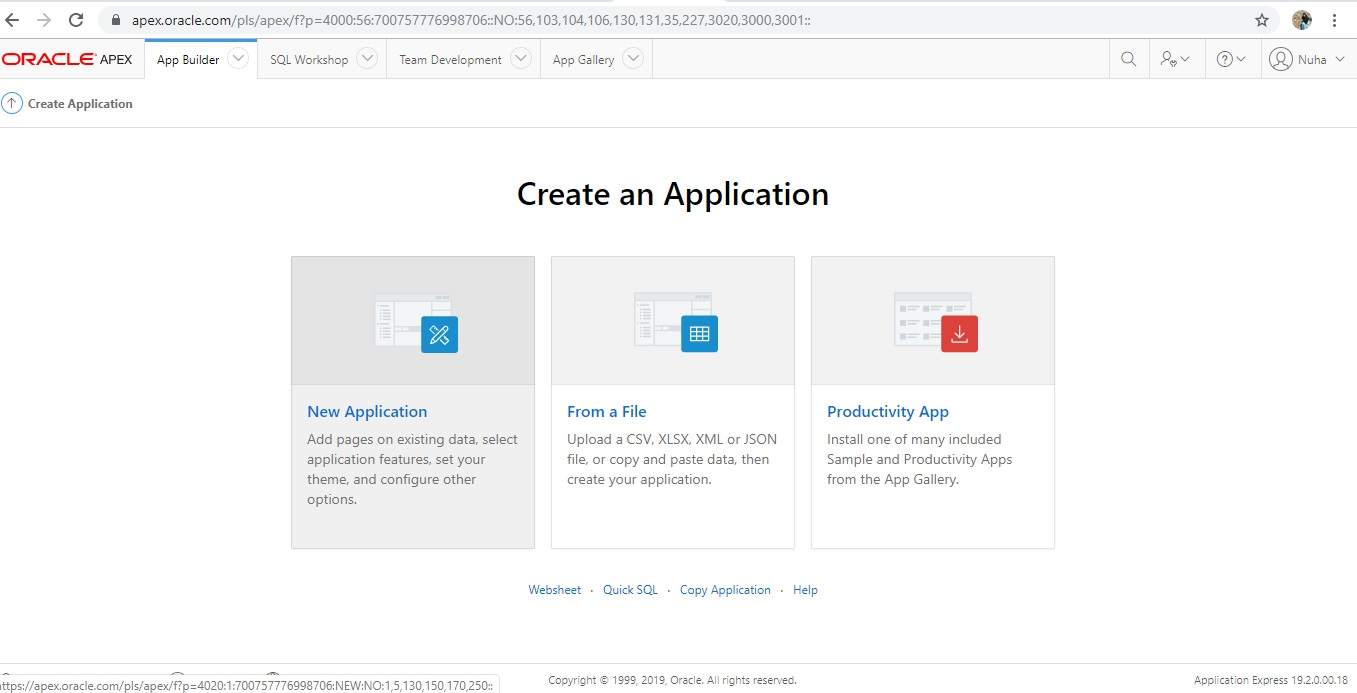
\includegraphics[width=11cm\textwidth]{figure/new app.jpg}
    \end{center}
    \item Pada tahapan ini kita Create Aplication dengan memasukkan nama aplikasi yang akan kita buat. Pada Tugas Besar kali ini saya membuat Aplikasi Stok Toko Aksesoris. 
    \begin{center}
    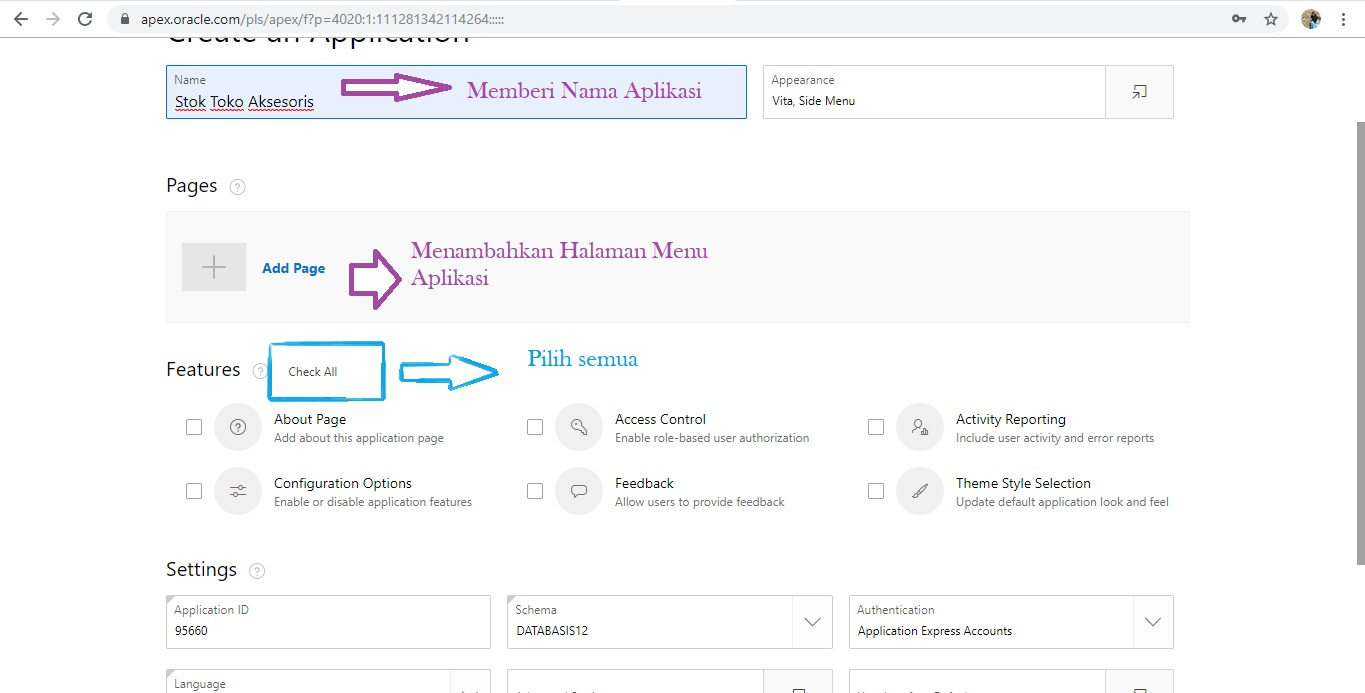
\includegraphics[width=11cm\textwidth]{figure/create app.jpg}
    \end{center}
     Beralih kita ke line perintah bawahnya yaitu Add Pages yaitu menambahkan halaman apa saja yang ada dalam aplikasi? Disini saya menambahkan 2 Halaman Yaitu Stok dan Produk.
     Cara menambahkan halaman yaitu dengan klik add page lalu pilih Interactive Report Lalu isi Page Name. disini say isi 'Stok' kita dapat menambahkan icon halaman pada icon set icon. Beralih pada table bawahnya ialah kita masukkan table untuk halaman stok yaitu 'table stok' yg telah kita buat sebelumnya. Gambar Contoh pada Add Page:
    \begin{center}
    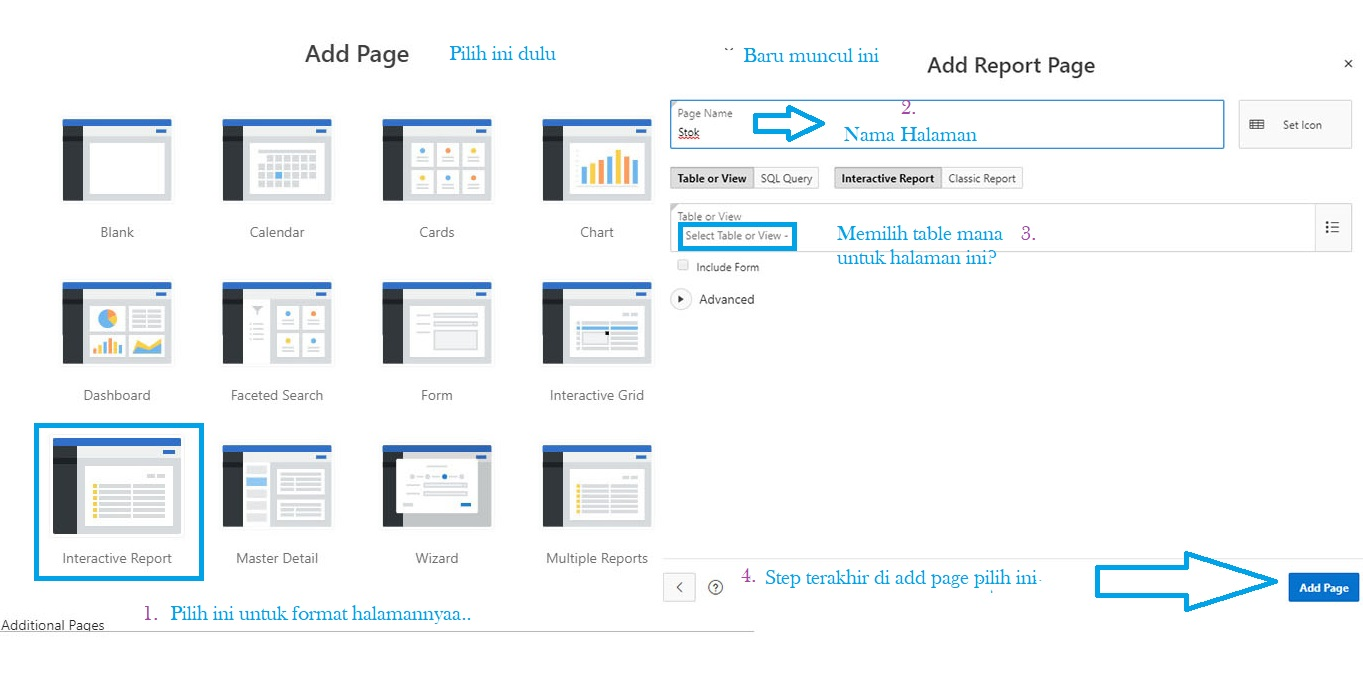
\includegraphics[width=11cm\textwidth]{figure/addpagenya.jpg}
    \end{center}
    langkah dalam add page tetapi itu baru satu table untuk satu halaman. Nah karena saya ada dua table saya ulangi add page lagi tetapi dengan nama halaman dan tentunya table yang berbeda yaitu halaman produk dengan table tambah produk.
    \item Jangan lupa klik Check All lalu Create Aplication.
    \item Aplikasi berhasil terbuat. Untuk menjalankan Aplikasi pilih Run
    \begin{center}
    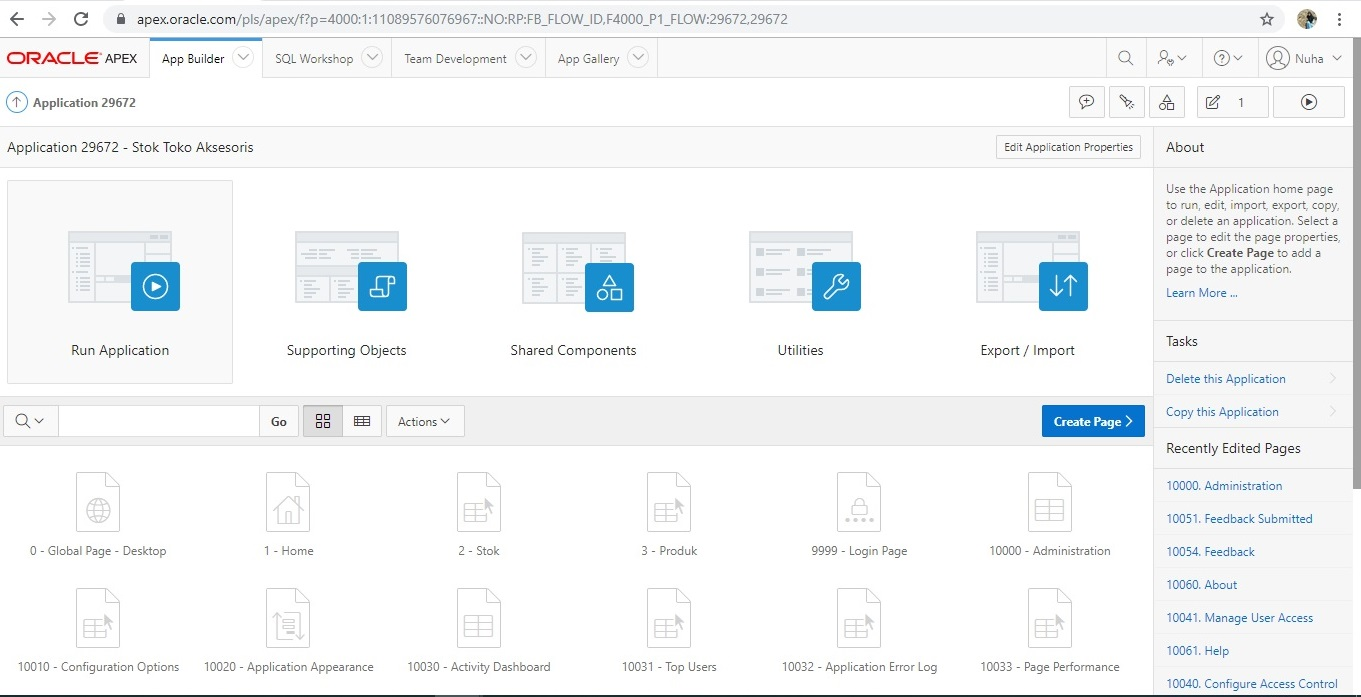
\includegraphics[width=11cm\textwidth]{figure/run.jpg}
    \end{center}
    \item Setelah kita pilih run kita akan diarahkan pada halaman login menggunakan user credensial anda. kita masukkan username dan passwors seperti pertama kali login Orecle APEX. Tampilan login aplikasi:
    \begin{center}
    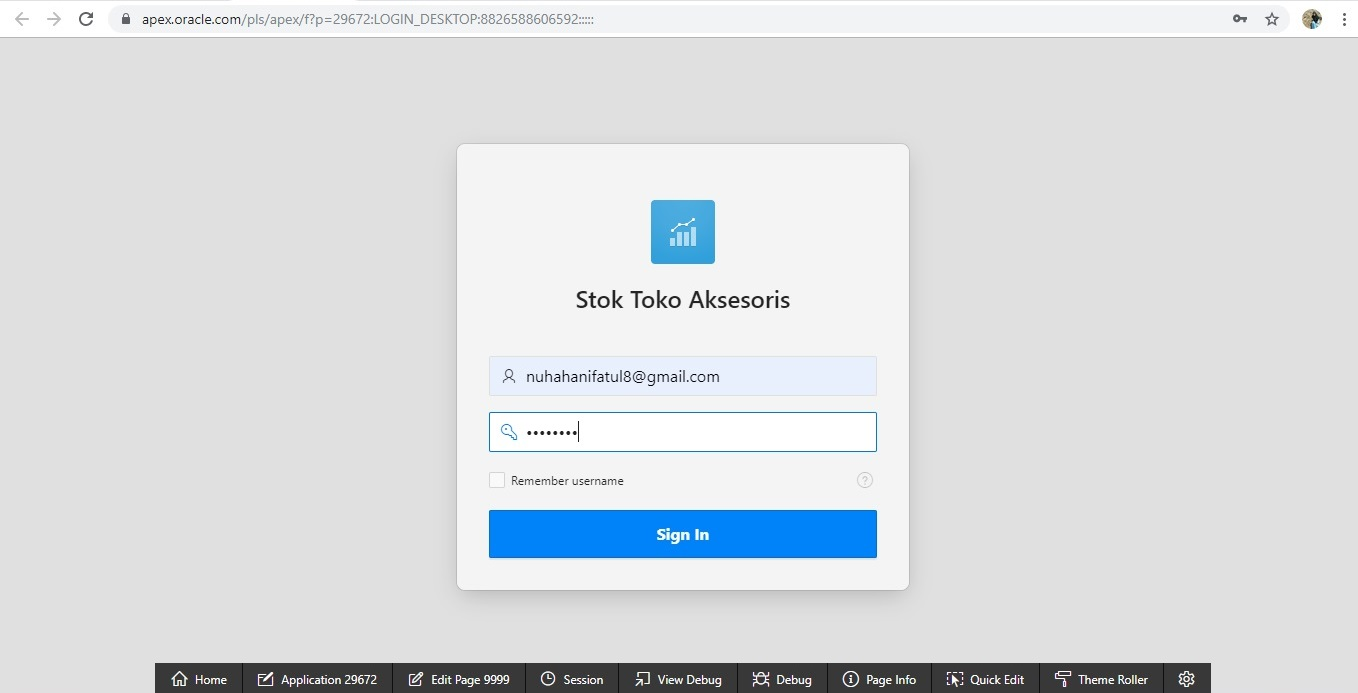
\includegraphics[width=11cm\textwidth]{figure/logins.jpg}
    \end{center}
    \item Jika kita berhasil login kita akan diarahkan pada tampilan aplikasi kita. Alhamdulillah ini adalah langkah terakhir. Seperti ini aplikasi saya.
    \begin{center}
    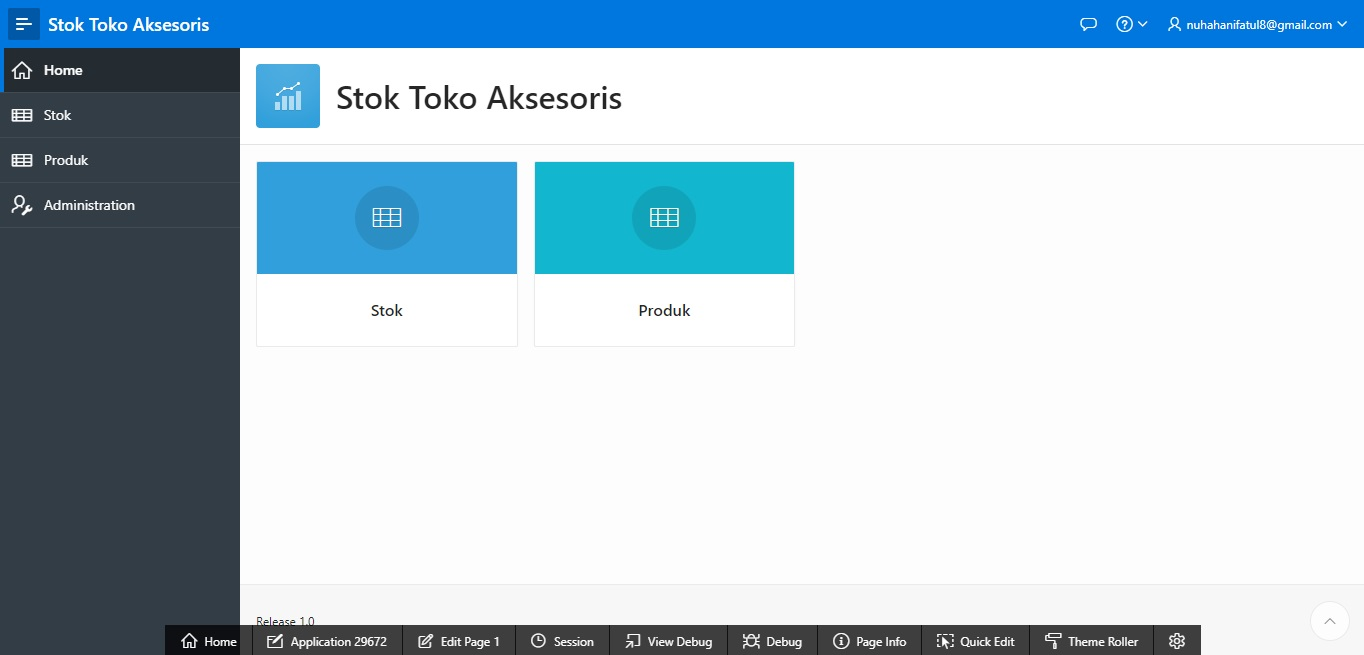
\includegraphics[width=11cm\textwidth]{figure/Stok Toko Aksesoris.jpg}
    \end{center}
\end{enumerate}
Workspace : databasis12 \\
Username : nuhahanifatul8@gmail.com \\
Password : anandra4 \\
link : https://apex.oracle.com/pls/apex/f?p=29672:1:8826588606592::NO:::
\end{document}
